\section{Specifications}
\label{sec:Specifications}

\newcounter{rulei}[subsection]
\newcommand{\rcnii}{\stepcounter{rulei}\arabic{section}.\arabic{subsection}.\arabic{rulei}}
\renewcommand{\labelenumi}{\rcnii}

\subsection{Markers}
\label{sub:markers}
The arena, tokens and robots involved in the game are labelled with \textit{libkoki} markers.
Each marker pattern encodes a number.
Each marker number is associated with a particular feature within the arena, and also has an associated size.
The marker numbers and sizes are as follows:

\begin{center}
  \begin{tabular}{lcc}
    \toprule
    \textbf{Item} & \textbf{Marker Numbers} & \textbf{Marker Size (mm)} \\
    \midrule
    Arena boundary & {} 0 -- 27 & 250 \\
    Robots & 28 -- 31 & 100 \\
    Token tops & 32 -- 40 & 250 \\
    Token bottoms & 41 -- 49 & 250 \\
    Token sides & 50 -- 61 & 250 \\
    \bottomrule
  \end{tabular}
\end{center}

% TODO: do we want each token to be unique identifiable?
%       If so we need at least 54 unique markers, which is doable, plus some for spares (and this footnote).
%       If not then we can drop this footnote and simplify the later rules table mapping marker numbers to tokens.
\footnotetext{The range of available token marker numbers is intentionally greater than the number required in the arena (see section~\ref{sub:Tokens}).  This makes replacing damaged tokens at the competition quicker.}

Two sets of marker codes will be used: one for development purpose, and one for the competition itself.
The competition set is only to be used inside the Student Robotics arena at the Student Robotics competition.
This is so that people carrying markers past the arena do not confuse robots.
The competition codes are 100 above the development codes.
When run in competition mode, the software provided by Student Robotics will subtract 100 from the detected marker codes, as well as ignore the development codes.

The markers can be printed on a black-and-white printer.
Marker designs can be downloaded from the documentation section of the Student Robotics website.

Unless specified otherwise, all markers described in this document are oriented vertically such that the principle corner of the marker (which is indicated by a dark grey dot in the black marker border) is on the higher edge.

\subsection{Robot Badges}
\label{sub:robot-badges}

\begin{figure}
  \centering
  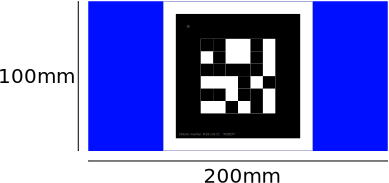
\includegraphics[width=\textwidth]{./images/robot-marker.pdf}
  \caption{An example robot badge.
           The blue areas shown are the human-compatible areas.
           All dimensions are in millimetres.}
  \label{fig:example-badge}
\end{figure}

\begin{enumerate}
\item A ``robot badge'' is a removable identifier that will be attached to a robot throughout a match.
      It features the robot's assigned marker for the match, as well as human-compatible areas to allow spectators to easily associate a robot with its starting location.
      An example of one of these badges is shown in figure~\ref{fig:example-badge}.
      The markings in the human-compatible areas are intentionally not specified.

\item A robot must feature four of the badge mounts shown in figure~\ref{fig:badge-mounting}.
      These mounts must permit a flat $200 \times 100mm$ panel to be attached to them.
      The three areas of each mount must feature the illustrated areas of hook-type Velcro to allow this panel to be fitted.

\item The four badge mounts must be on the exterior of the robot, parallel with the vertical plane, and should be perpendicular to each other about the vertical axis\footnote{Teams can apply for a team-specific rule alteration to the required number of badges.
      Clear justification must be provided by the team with such a request.}
      The orientation of the badge mounts is unimportant, but teams are encouraged to position them horizontally as shown in figure~\ref{fig:example-badge}.

\item The mapping between a given robot and its robot badge is as follows:

\begin{center}
  \begin{tabular}{cc}
    \toprule
    \textbf{Corner} & \textbf{Marker Number} \\
    \midrule
    0 & 28 \\
    1 & 29 \\
    2 & 30 \\
    3 & 31 \\
    \bottomrule
  \end{tabular}
\end{center}

\begin{figure}
  \centering
  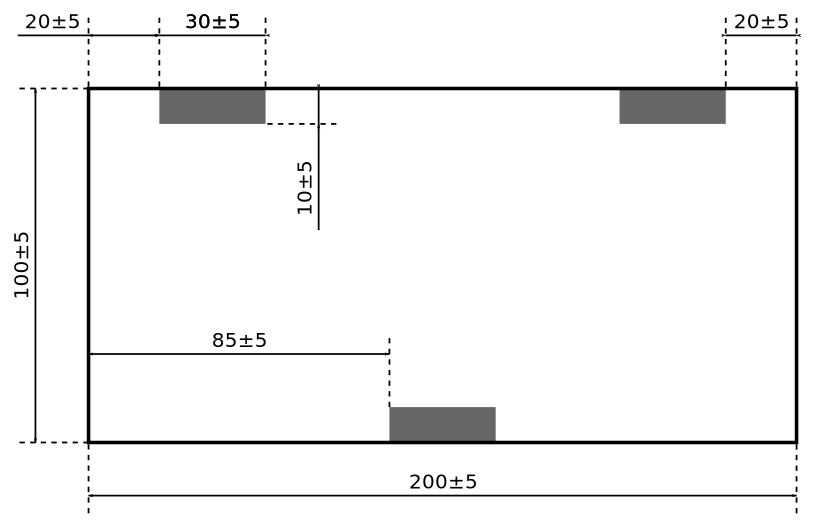
\includegraphics[width=\textwidth]{./images/badge-mounting.pdf}
  \caption{The dimensions of the required robot badge mountings.
           The shaded areas are hook-type Velcro.
           All dimensions are in millimetres.}
  \label{fig:badge-mounting}
\end{figure}

\end{enumerate}

\subsection{Arena}
\label{sub:arena}
\begin{enumerate}
\item The match arena floor, overall, is an $8m \times 8m$ square, as shown in figure~\ref{fig:arena-dim}.
      The tolerance of these two dimensions is $\pm0.2m$.

\begin{figure}
  \centering
  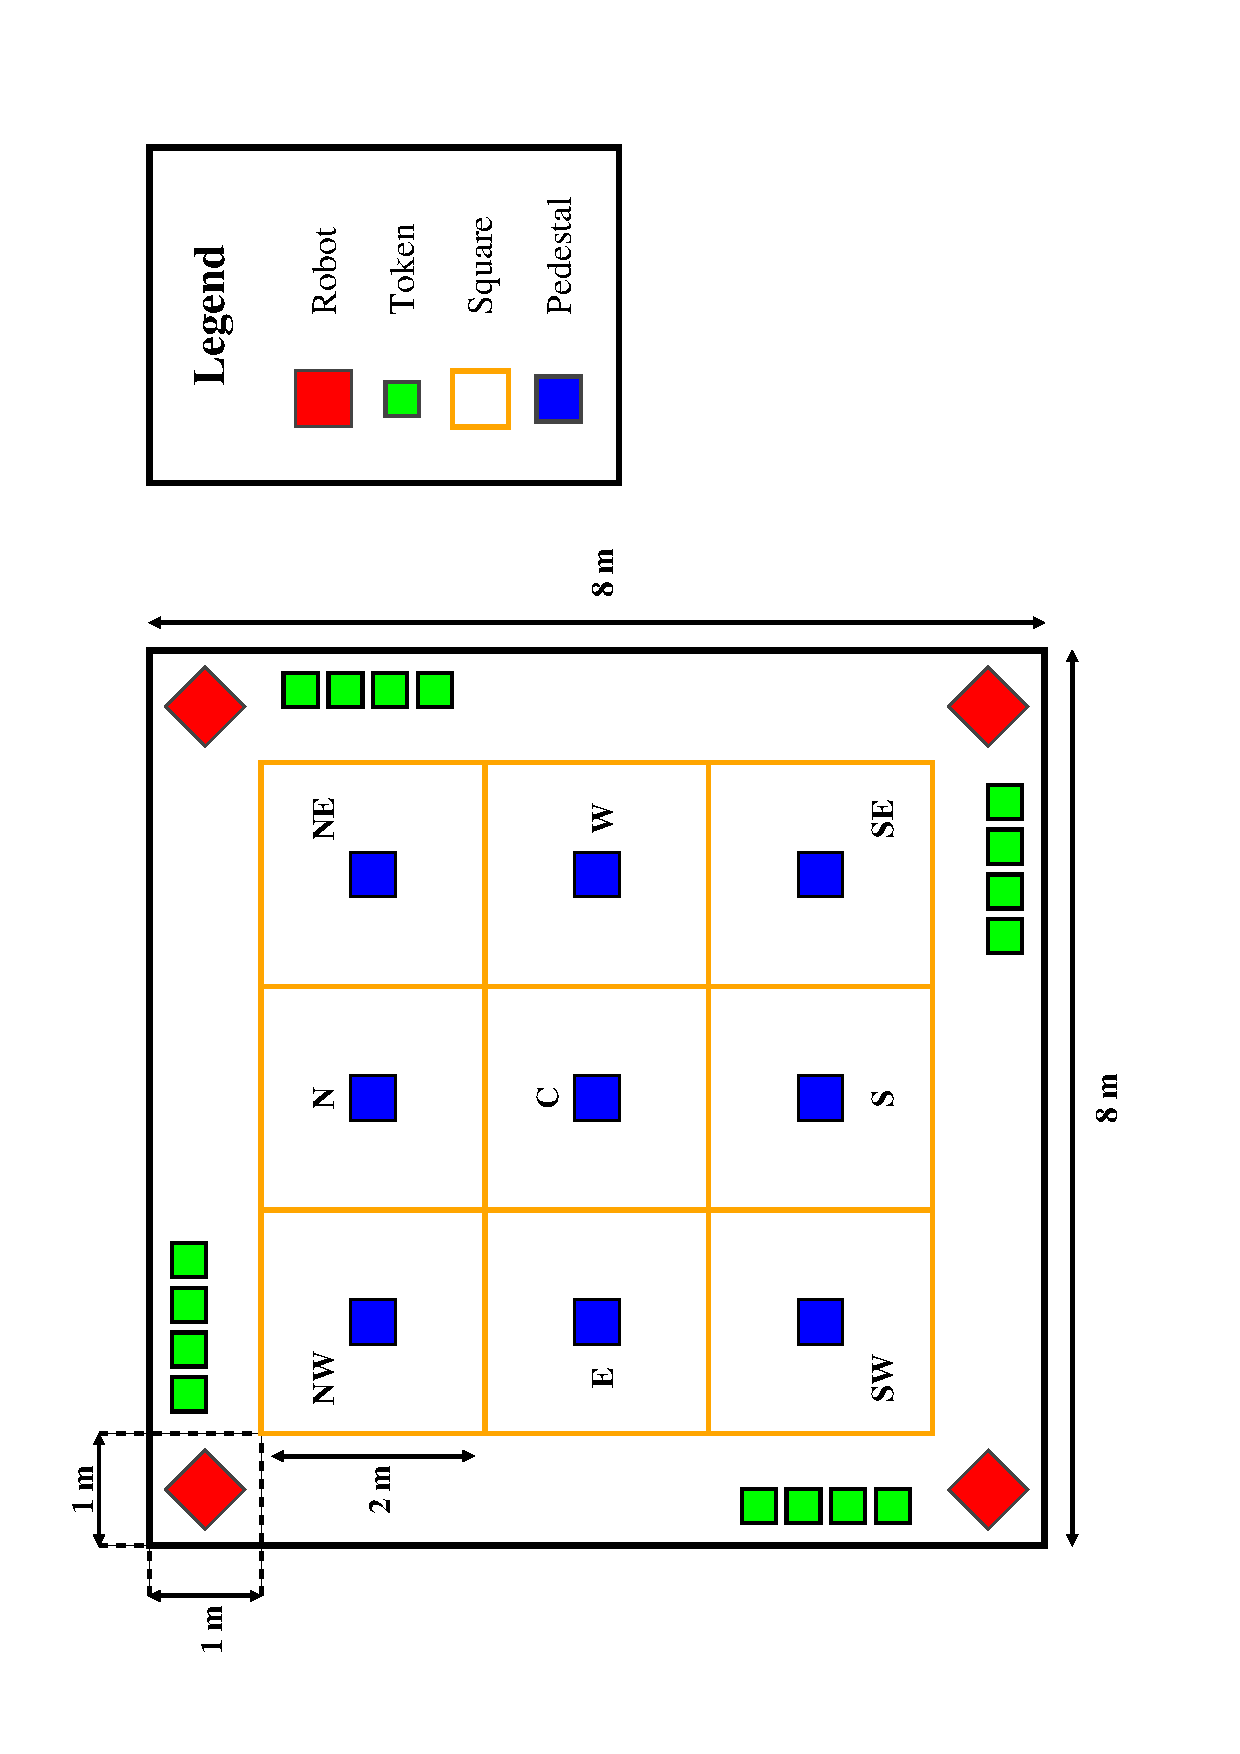
\includegraphics[width=\textwidth]{./images/arena.pdf}
  \caption{\label{fig:arena-dim}A bird's-eye view of the arena. All dimensions are in millimetres.}
\end{figure}

\item The floor of the arena is covered with a closed-loop, short pile carpet.

\item The perimeter of the arena floor is delimited by the arena wall, which has a minimum height of $100mm$.

\begin{figure}
  \centering
  
\includegraphics[width=\textwidth]{./images/sidewall.pdf}
  \caption{Seven $250mm$ wide markers are spaced evenly along each $8m$ arena wall.
           The markers are placed $50mm$ above the floor.
           All dimensions are in millimetres.}
  \label{fig:arena-wall}
\end{figure}

\begin{figure}
  \centering
  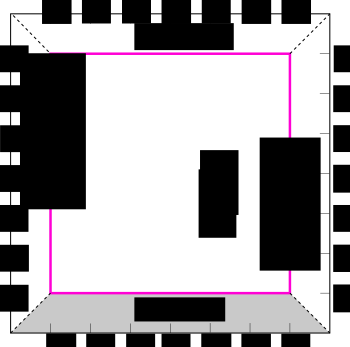
\includegraphics[width=0.5\textwidth]{./images/arena-markers.pdf}
  \caption{Twenty eight arena wall markers are positioned around the perimeter of the arena with the marker codes incrementing in a clockwise fashion.
           The corners are counted in a clockwise fashion, with corner 0 being the corner closest to arena marker 0.}
  \label{fig:arena-zones}
\end{figure}

\item Each wall of the arena features seven $250mm$ libkoki markers.
      Figure~\ref{fig:arena-wall} shows the positioning of these markers, whilst figure~\ref{fig:arena-zones} shows the numbering of these markers.

\item Each robot will be assigned a corner at the start of every match to indicate its starting position.
      Corner starting positions are $1000 \pm 20mm$ square and will be marked by $25mm$ paper-based masking tape.
      The mapping of these corner numbers in the arena is shown in figure~\ref{fig:arena-zones}.

\item Student Robotics reserves the right to have match officials in the arena during games.

\end{enumerate}


\subsection{Scoring Zones}
\label{sub:Zones}

\begin{enumerate}
\item There are four zones in the arena, one in each of the corners.
      The arrangement and dimensions of these zones can be seen in figure~\ref{fig:arena-dim}.

\item Where the boundary of a scoring zone is not formed by the arena wall it will be marked by $25mm$ tape.
\end{enumerate}

\subsection{Tokens}
\label{sub:Tokens}
\begin{enumerate}
\item Tokens are cubic cardboard boxes with a side length of $250 \pm 10 mm$.

\item Each token will be assigned a unique combination of $200mm$ libkoki markers.

\item Token side markers will be:
    \begin{enumerate}
    \item Oriented such that the top left corner of each marker (identified by a small grey dot) is affixed to the top left of a token's side face.

    \item Assigned to a team in one of the four corners.
          The lowest numbered side marker will always correspond to corner 0, the second lowest to corner 1, the third to corner 2 and the highest to corner 3.

    \item Arranged in one of three nets, ensuring that the pairs of opposing sides of the tokens are spread evenly over all pairwise combinations.
          The arrangements are shown in figure~\ref{fig:token-nets}.
    \end{enumerate}

\begin{figure}
  \centering
  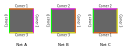
\includegraphics[width=\textwidth]{./images/token-nets.pdf}
  \caption{Tokens' sides are arranged into one of three nets.
           The arrangements of each of the nets is shown as viewed from \textit{above} a constructed token.}
  \label{fig:token-nets}
\end{figure}

\item There will be 9 tokens in the arena, 3 of each net.
      Their general starting positions can be seen in figure~\ref{fig:arena-dim}.
      The starting position of each net are not defined.

\item Most tokens will start with their top facing upwards.
      % TODO: What's the point of doing this -- surely all it means is that everyone starts with more points, which doesn't achieve anything?
      The four nearest the corner zones will instead have the face corresponding to the nearest corner facing upwards.

\item The assignment of marker numbers to nets is as follows:
\begin{center}
  \begin{tabular}{cccc}
    \toprule
    \textbf{Net} & \textbf{Top Marker} & \textbf{Bottom Marker} & \textbf{Side Markers} \\
    \midrule
    A & 32 & 41 & 50 -- 53 \\
    A & 33 & 42 & 54 -- 57 \\
    A & 34 & 43 & 58 -- 61 \\
    B & 35 & 44 & 62 -- 65 \\
    B & 36 & 45 & 66 -- 69 \\
    B & 37 & 46 & 70 -- 73 \\
    C & 38 & 47 & 74 -- 77 \\
    C & 39 & 48 & 78 -- 81 \\
    C & 40 & 49 & 82 -- 85 \\
    \bottomrule
  \end{tabular}
\end{center}

\item The sides of the token will be adorned in similar human-compatible markings as the robot badges are.

\end{enumerate}

\clearpage
